\setSection{3}
\section{The Central Limit Theorem}

The reason Normal distributions play an outsized role in applied statistics is that the distribution of  $\bar{Y}$ can be made \emph{nearly normal}, no matter the underlying distribution of $Y$ (Does not need to start \say{life} Normal). So \emph{nearly} normal, that we just pretend it is.



\nnl \textbf{Theorem 7.4: The Central Limit Theorem (CLT)}

\nl Let $\yn$ be independent and identically distributed (iid) random variables with
$$\E{Y_i} = \mu \wideand \Var{Y_i} = \sigma^2 < \infty$$
(Need finite variance for CLT to hold)

\nl Define $$U_n = \frac{\bar{Y}-\mu}{\sqrt{\frac{\sigma^2}{n}}} = \frac{\sum (Y_i) - n\mu}{\sigma \sqrt{n}}.$$

\nl The CLT says the distribution function of
$U_n$ converges to $N(0,1)$ as $n\to\infty$.

\nl Big idea: The distribution $\Ybar$ can be thought of as $\normalDist{\mu}{\frac{\sigma^2}{n}}$.

\defn The \bu{support of $f$} is the domain on which $f$ is non-zero.

\example* Let $\Xbar$ denote the mean of a random sample of size $n=15$, from the distribution whose pdf is $$f(x) = \frac{3}{2}x^2, \qquad x \,\in\, [-1,1]$$


\nl Can be shown that
$$\mu = \Eb{X} = 0 \wideand \sigma^2 = \Eb{(X-\mu)^2} = \frac{3}{5}$$

\nl To compute $\P{0.03 \leq \Xbar \leq 0.15}$, we use the CLT and assume $\Xbar$ is distributed  by
$$\normalDist{\mu}{\frac{\sigma^2}{n}} = \normalDist{0}{\frac{3/5}{15}} = \normalDist{0}{\over{25}}.$$

\nl Then
\begin{align}
    \P{0.03 \leq \bar{X} \leq 0.15} &= \P{\frac{0.03-\mu}{\sigma} \leq \frac{\Xbar - \mu}{\sigma} \leq \frac{0.15-\mu}{\sigma}} \notag\\
    &= \P{\frac{0.03-0}{\sqrt{1/25}} \leq Z \leq \frac{0.15-0}{\sqrt{1/25}}} \notag\\
    &= \P{\frac{0.03}{\sqrt{1/25}} \leq Z \leq \frac{0.15}{\sqrt{1/25}}} \notag\\
    &= \P{0.15\leq Z \leq 0.75} \notag\\
    &= \text{Table4}(0.15) - \text{Table4}(0.75)\notag\\
    &= 0.4404 - 0.2266 \notag\\
    &= 0.2138 \notag
\end{align}
\recall Table 4 gives \underline{upper} tail probabilities.

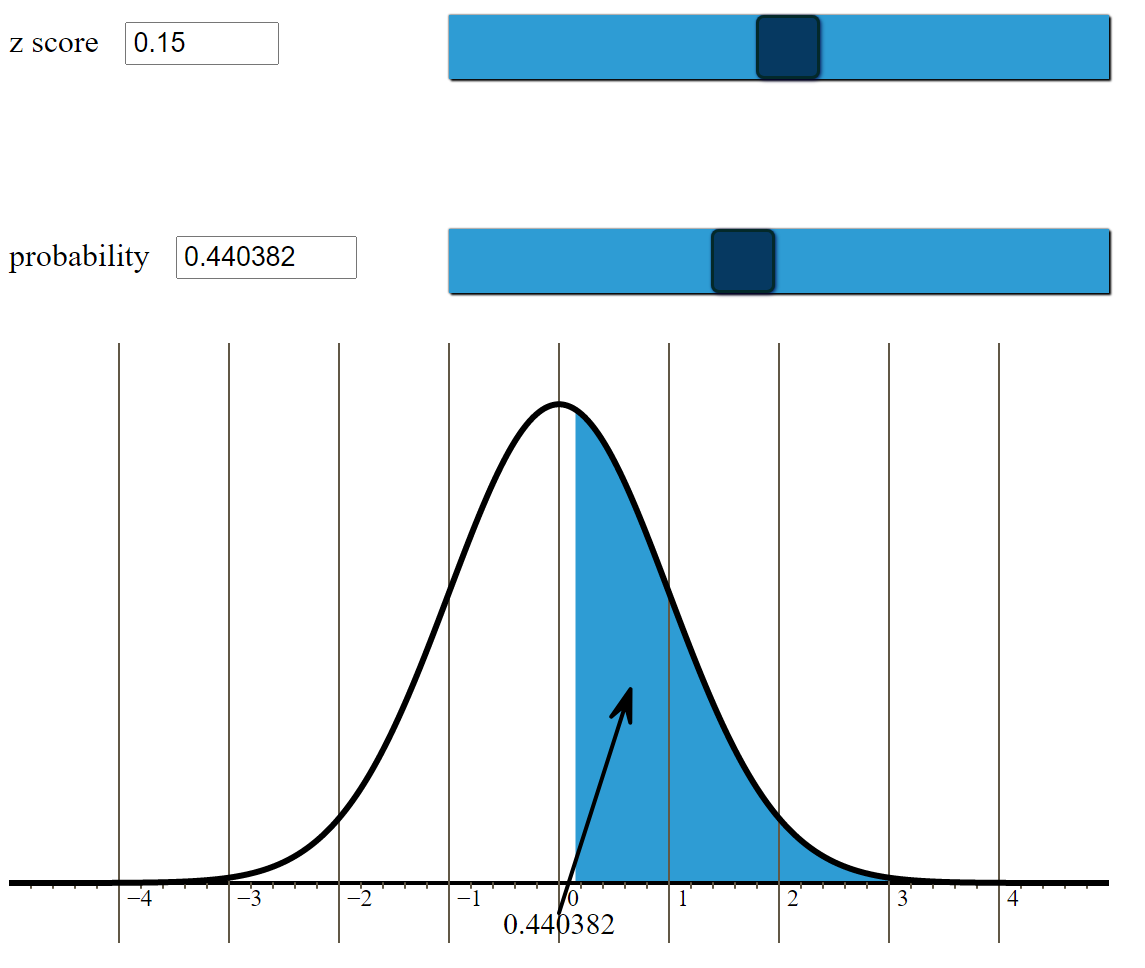
\includegraphics[width=3in]{z 0.15.PNG}
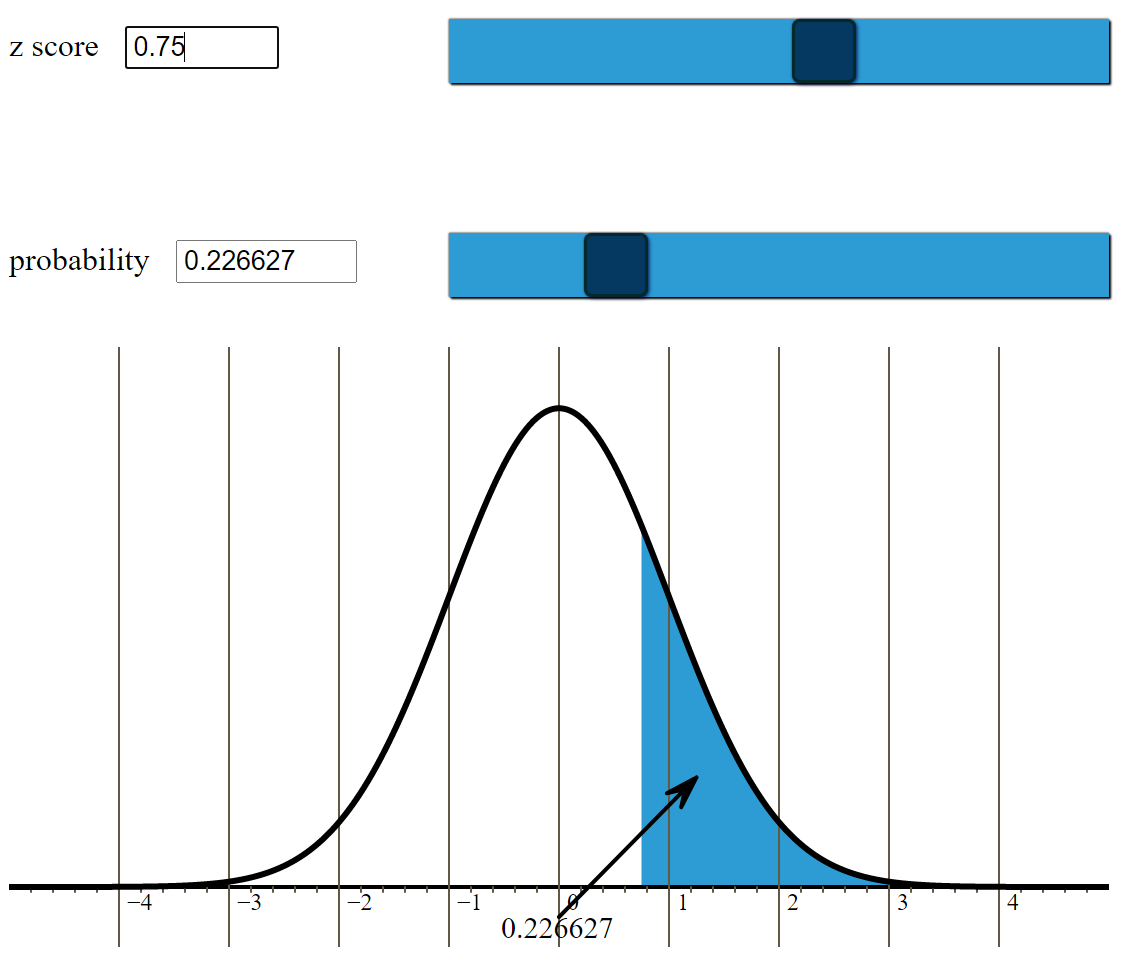
\includegraphics[width=3in]{z 0.75.PNG}

\nl Therefore, 
\begin{align*}
    \text{Table4}(0.15) - \text{Table4}(0.75) &= \P{Z > 0.15} - \P{Z > 0.75}\\ &= 0.4404 - 0.2266 \\ &= 0.2138
\end{align*}

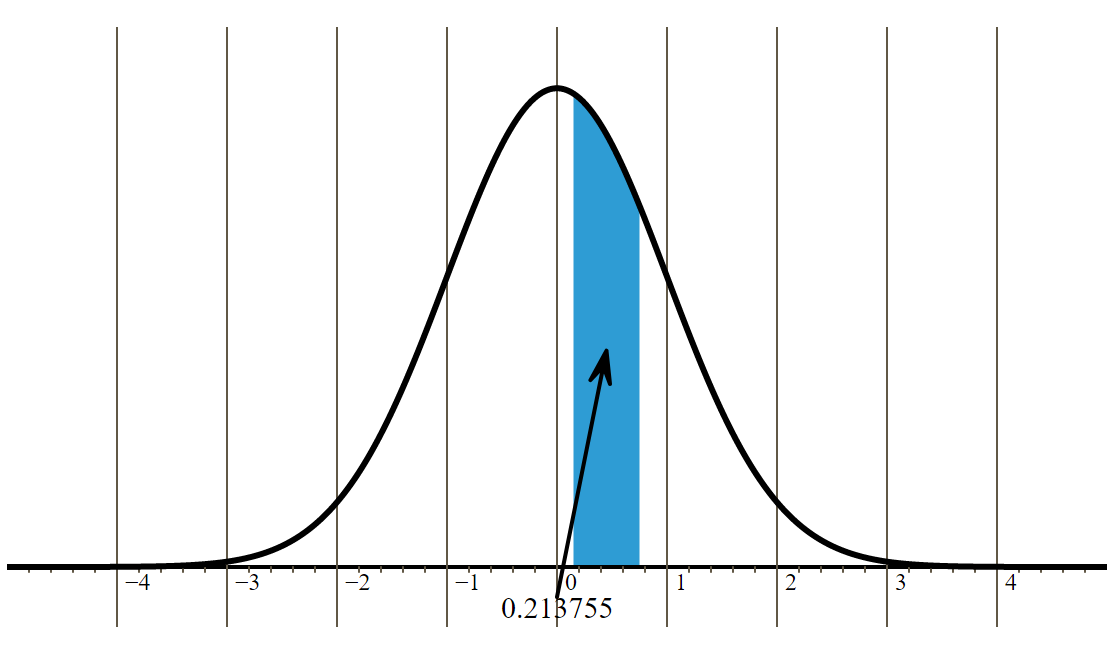
\includegraphics[width=6.25in]{7_4 normal area.PNG}

\disc* About $n$. Suprisingly, \say{large} $n$ doesn't need to be that large.\\Usually for any random variable $X$ and any distribution, then
$$\boxed{n \geq 30 \quad \text{is enough.}}$$

\noindent
That is, when $n \geq 30$, the CLT says $\normalDist{\mu}{\frac{\sigma^2}{n}}$ yields a good approximation of $\Xbar$.

\nl When $X$ is symmetric, unimodal, and continuous, $n = 4$ or $n = 5$ is often enough. 

\newpage
\addcontentsline{toc}{subsection}{Table 4: Normal Curve Areas}
\noindent\begin{center}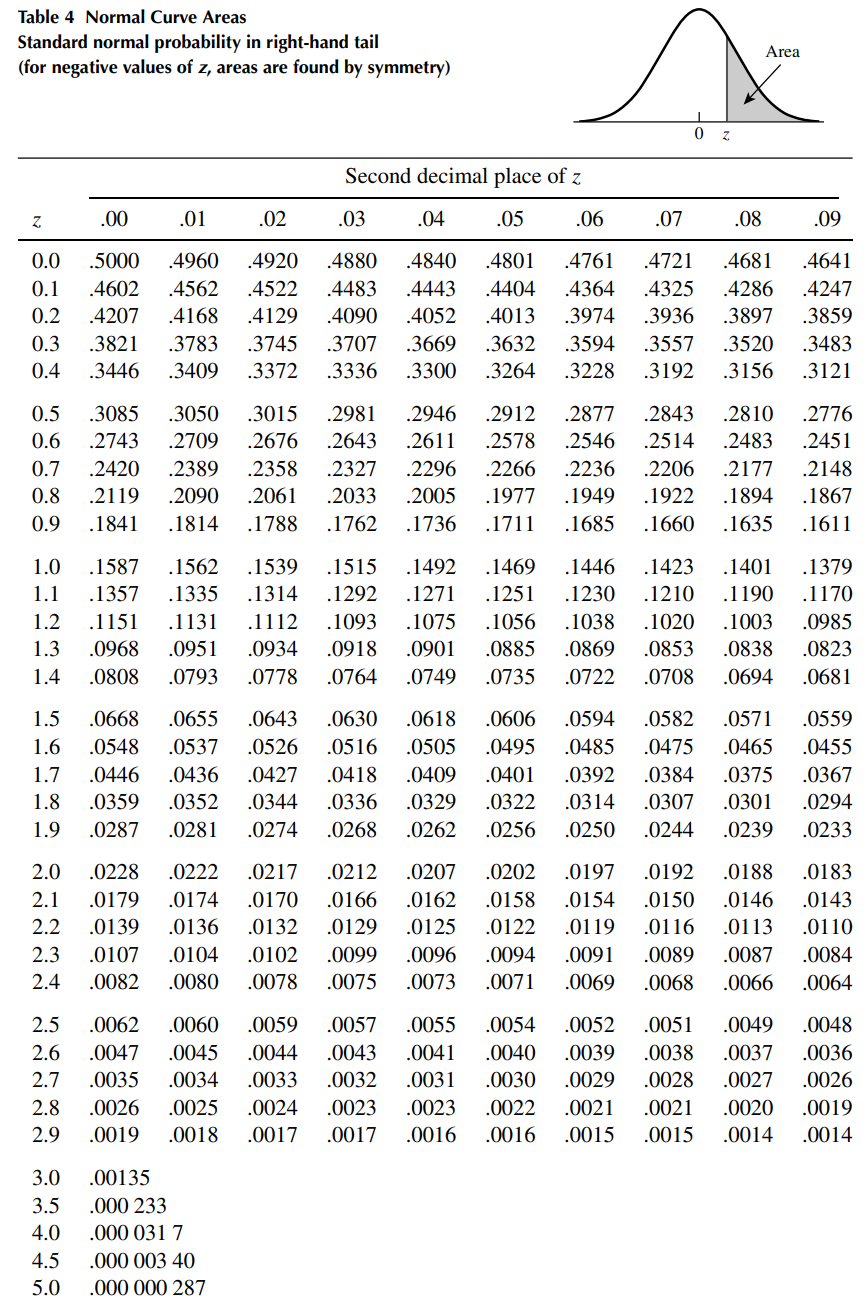
\includegraphics[width=6in]{Table4.png}
\end{center}